\section{Experiment 10H-G: global measured-output prediction-error gate}
\label{sec:experiment10hg}

\paragraph{Purpose.}
Experiments 10H-E and 10H-F showed that neither generic innovation summaries
nor first-order scores at a fixed nominal model reliably reveal the latent
vehicle groups. Before attempting a mixture or federated EM method,
Experiment 10H-G asks a narrower prerequisite question: can one structured
global LPV model be learned reliably from measured input--output trajectories
without true states, physical parameters, matrices, or class labels?

The nine effective coordinates and structured $A(v;\theta),B(v;\theta)$ model
from 10H-F are retained. A steady-state KF produces normalized innovations
from measured yaw rate, lateral acceleration, applied steering, steering
command, and speed. The objective is the mean squared normalized innovation.
The fit uses 20 clients per fleet; every third client is held out by list
position, giving ten label-blind held-out clients. Each development fleet is
optimized from three physically bounded initializations. The best training
solution is evaluated on the untouched clients. Conditional profiles perturb
each fitted log-coordinate by $\{-0.16,-0.08,0,0.08,0.16\}$ while holding the
others fixed.

The bounds are fixed multipliers, 0.35 and 3.0, of one public nominal design;
they do not use the simulated client truths. Class labels and hidden physical
parameters are opened only after fitting for retrospective interpretation.
Seeds 611--620 remain sealed.

\paragraph{Prediction result.}
The learned model improves held-out normalized prediction error in every
development fleet. The improvement ranges from 9.50\% to 21.86\%, with a mean
of 15.76\%. Thus measured outputs contain useful information beyond the
nominal observer, and the structured global-fit direction is not rejected on
predictive grounds.

\paragraph{Optimization and identifiability result.}
The stronger optimizer gate fails. Every selected run reaches the declared
25-iteration limit, so the optimizer-success rate is zero. Across the three
starts, the worst objective spread is 4.70\% and the worst coordinate
coefficient of variation is 0.330, both above the declared tolerances of
0.5\% and 0.08. Three of five selected fits place one of nine coordinates on a
bound. The minimum conditional edge increase is $-0.057$\%, meaning that at
least one selected point is not even a coordinate-wise minimum at the audited
profile radius. Retrospectively, the fitted vector has mean log-RMSE 0.641
relative to the arithmetic mean of the training clients' effective truths.
That diagnostic is not used for fitting or gate decisions.

\begin{table}[htbp]
\centering
\caption{Experiment 10H-G development diagnostics.}
\label{tab:experiment10hg}
\begin{tabular}{lr}
\toprule
Diagnostic & Result\\
\midrule
Mean held-out prediction improvement & 15.76\%\\
Minimum held-out prediction improvement & 9.50\%\\
Optimizer success rate & 0/5\\
Maximum restart objective spread & 4.70\%\\
Maximum restart coordinate CV & 0.330\\
Minimum conditional-profile edge increase & $-0.057$\%\\
Maximum bound-active fraction & 1/9\\
Development gate & Fail\\
\bottomrule
\end{tabular}
\end{table}

\begin{figure}[htbp]
\centering
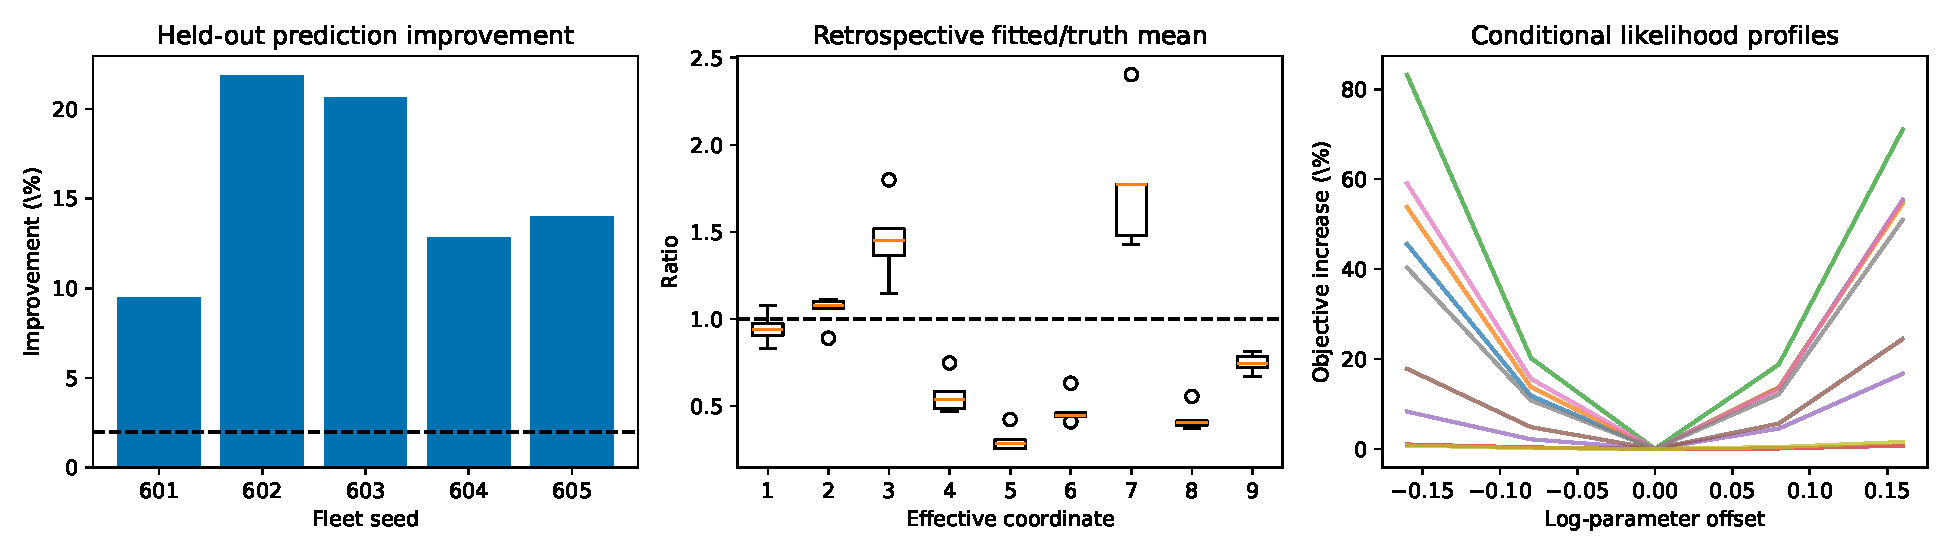
\includegraphics[width=0.98\linewidth]{../results/figures/experiment_10hg_global_prediction_error.pdf}
\caption{Held-out prediction improvement, retrospective fitted-to-fleet-mean
ratios, and conditional objective profiles for the global structured fit.}
\label{fig:experiment10hg}
\end{figure}

\paragraph{Decision.}
The positive held-out result and failed optimizer gate must not be conflated.
They establish that raw-output fitting is informative, but not that the
nine-coordinate solution is unique or sufficiently reproducible to seed a
mixture. Starting multi-model EM now would mix physical grouping with
initialization artifacts and weak directions.

The next experiment should therefore repair the $K=1$ estimator before any
clustering: introduce exact or automatic-differentiation gradients, scale the
coordinates using the 10H-F information matrix, and compare a staged fit
(actuator/relaxation dynamics followed by force/yaw coefficients) with the
joint fit. A successful repair must converge before its iteration budget,
collapse restart dispersion, retain held-out improvement, avoid active
bounds, and show positive local profile curvature. Only then is a known-$K$
joint membership/model experiment warranted.

\paragraph{Reproducibility.}
The preregistered configuration and implementation are in
\path{code/config/experiment_10hg.json} and
\path{code/experiments/experiment_10hg_global_prediction_error.py}. Per-fleet
summaries, fitted coordinates, restart outcomes, profile values, gate
decisions, leakage declaration, and provenance hashes are stored under
\path{results}.
